% begin module cylindrical-shells-ex
\begin{frame}
\begin{example}
\begin{columns}
\column{0.6\textwidth}
\begin{pspicture}(-1,-2)(3,3)%
\tiny%
\renewcommand{\fcScreenStyle}{x}%
\fcBoundingBox{-2.2}{-1.2}{2.5}{2.5}%
\renewcommand{\fcScreen}{[0 0 -1] 0}%
\renewcommand{\fcIterationsU}{4}%
\only<handout:2|5->{\renewcommand{\fcScreen}{[-0.07 dup -1] 0}}%
\only<handout:2|6->{\renewcommand{\fcScreen}{[-0.14 dup -1] 0}}%
\only<handout:2|7->{\renewcommand{\fcScreen}{[-0.21 dup -1] 0}}%
\only<handout:2,3|8->{\renewcommand{\fcScreen}{[-0.28 dup -1] 0}}%
\newcommand{\theFun}{u u mul 2 mul u u u mul mul sub\space}%
\newcommand{\theYAxis}{0\space}%
\newcommand{\theSurfaceFla}{v cos u mul \theFun v sin u mul\space}%
\newcommand{\theSurface}{%
\fcSurfaceInScene[colorVU= {1 0.5 0.5}, iterationsU=6, arrows=none, linewidth=0.3, linecolor=black ]{0.03}{0}{1.99}{30 \fcIterationsV\space mul}{[\theSurfaceFla]}{}%
}%
\uncover<handout:1|4-8>{\pscustom*[linecolor=\fcColorAreaUnderGraph]{%
\fcLineIIId{ [0 0 0]}{[2 0  0]}%
\fcCurveIIId{2}{0}{[1 dict begin /u t def t \theFun 0 end]}%
}}%
\fcStartIIIdScene%
\fcAxesIIIdInScene[zLabel={}, arrows=->]{2.2}{2.2}{3}%
\uncover<handout:2,3|8->{\fcPutIIId[t]{[0 0 3.1]}{$z$}}%
\only<handout:0|9>{%
\renewcommand{\fcIterationsV}{4}%
\theSurface%
}%
\only<handout:0|10>{%
\renewcommand{\fcIterationsV}{8}%
\theSurface%
}%
\only<handout:2|11,12, 24->{%
\renewcommand{\fcIterationsV}{12}%
\theSurface%
}%
\only<handout:2,3|12-23>{%
\fcSurfaceInScene[linewidth=1, arrows=(none), colorUV=cyan, colorVU=cyan, linecolor=blue, iterationsU=10, iterationsV=1]{0}{0}{360}{1 dict begin /u 0.9 def \theFun  end}{[u cos 0.9 mul v u sin 0.9 mul ]}{}%
\fcSurfaceInScene[linewidth=1, arrows=(none), colorUV=cyan, colorVU=cyan, linecolor=blue, iterationsU=10, iterationsV=1]{0}{0}{360}{1 dict begin /u 0.9 def \theFun  end}{[u cos 0.8 mul v u sin 0.8 mul ]}{}%
\fcSurfaceInScene[linewidth=1, arrows=(none), colorUV=cyan, colorVU=cyan, linecolor=blue, iterationsU=10, iterationsV=1]{0}{0.8}{360}{0.9}{[u cos v mul 0.891 u sin v mul ]}{}%
}%
\only<4->{\fcCurveIIIdInScene[linewidth=1, arrows=(none), linecolor= \fcColorGraph]{0}{2}{1 dict begin /u {t} def  [t \theFun 0] end}}%
\only<4->{\fcLineIIIdInScene[linewidth=1, arrows=(none), linecolor= \fcColorGraph]{[0 0 0]}{[2 0 0]}}%
\fcFinishIIIdScene%
\only<handout:1|2-3>{\fcCurveIIId{-0.8}{2.2}{1 dict begin /u {t} def  [t \theFun 0] end}}%
\only<handout:1|3>{\fcLineIIId[linecolor=\fcColorGraph]{[-0.8 0 0]}{[2.1 0 0]}}%
\uncover<handout:3|13->{ \fcLineIIId[linecolor=black, linewidth=0.4pt]{[0.9 -0.05 0]}{[0.9 0.05 0]}}%
\fcLineIIId[linecolor=black, linewidth=0.4pt]{[2 -0.05 0]}{[2 0.05 0]}%
\fcLineIIId[linecolor=black, linewidth=0.4pt]{[-0.05 1 0]}{[0.05 1 0]}%
\uncover<handout:3|13->{ \fcPutIIId[t]{[1 -0.1 0]}{$x$}}%
\fcPutIIId[t]{[2 -0.1 0]}{$2$}%
\fcPutIIId[r]{[-0.1 1 0]}{$1$}%
\only<2->{\fcPutIIId[b]{[4 3 div 1.5 0]}{$\alertNoH{15}{y=2x^2-x^3}$}}%
\only<handout:0|15,20>{\fcLineIIId[linecolor=red, linewidth=2pt]{[0.9 0 0]}{[0.9 dup 1 dict begin /u exch def \theFun end 0]}}%
\only<handout:0|22>{\fcLineIIId[linecolor=red, linewidth=2pt]{[0.9 0 0]}{[0.8 0 0]}}%
\only<handout:0|17,21>{\fcCurveIIId[linecolor=red, linewidth=2pt]{0}{360}{[t cos 0.9 mul 0 t sin 0.9 mul]}}%
\only<handout:0|22>{\fcLineIIId[linecolor=orange, linewidth=2pt]{[0.8 0 0]}{[0.9 0 0]}}%
\only<handout:0|25->{%
\fcLineIIId[linecolor=blue, linewidth=2pt]{[0 0 0]}{[2 0 0]}%
\fcDotIIId[linecolor=blue]{[0 0 0]}
\fcDotIIId[linecolor=blue]{[2 0 0]}
}%
\end{pspicture}
%\only<handout:0| -1>{%
%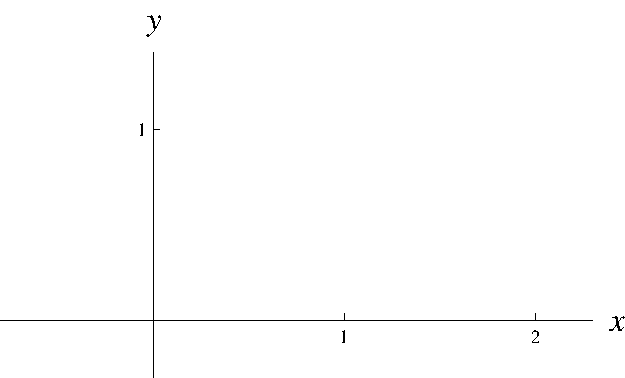
\includegraphics[width=3cm]{volumes/pictures/06-03-exa.pdf} %
%}%
%\only<handout:0| 2>{%
%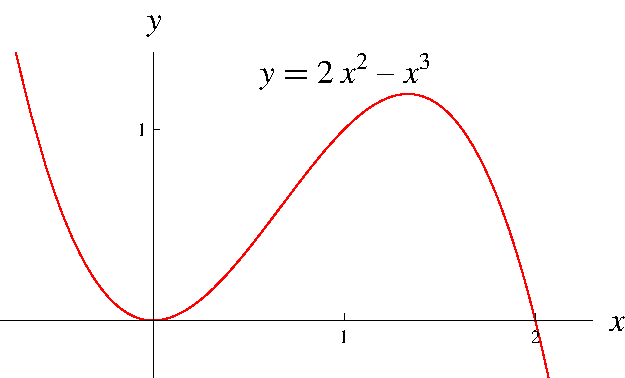
\includegraphics[width=3cm]{volumes/pictures/06-03-exb.pdf} %
%}%
%\only<handout:0| 3>{%
%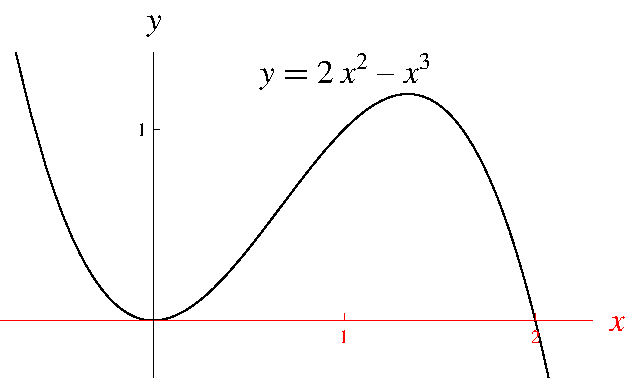
\includegraphics[width=3cm]{volumes/pictures/06-03-exc.pdf} %
%}%
%\only<handout:0| 4>{%
%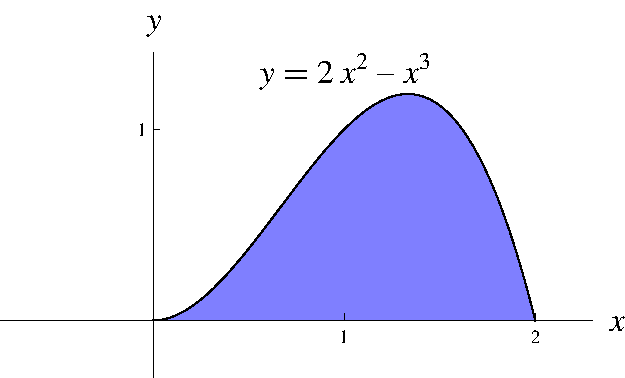
\includegraphics[width=3cm]{volumes/pictures/06-03-exd.pdf} %
%}%
%\only<5->{%
%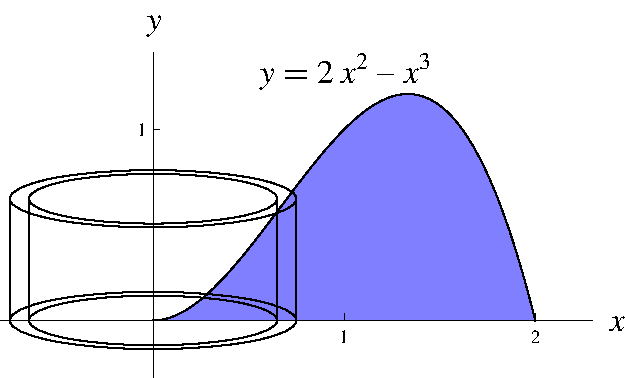
\includegraphics[width=3cm]{volumes/pictures/06-03-exe.pdf} %
%}%
\column{0.4\textwidth}
Find the volume of the solid obtained by rotating about the $y$-axis \alertNoH{4}{the region bounded by \alertNoH{2}{$y = 2x^2 - x^3$} and \alertNoH{3}{the $x$-axis}}.
\end{columns}
\uncover<handout:3|13->{Cylindrical shell: \alertNoH{13}{outer radius $x$}; \alertNoH{14,15,20}{height: $\fcAnswerUncover{13}{15}{2x^2-x^3} $}; \alertNoH{16,17,21}{circumference: $ \fcAnswerUncover{13}{17}{2\pi x }$}; \alertNoH{18,19,23}{ \alertNoH{22}{infinitesimal} volume: $\fcAnswerUncover{13}{19}{\alertNoH{21}{2\pi x} (\alertNoH{20}{2x^2-x^3}) \alertNoH{22}{\diff x}} $}.}

\uncover<handout:3|1->{
$\begin{array}{@{}r@{}c@{}l}
\uncover<23->{V & =&\displaystyle \int_{{\fcAnswer{25}{0}} }^{{ \fcAnswer{25 }{2}}} \alertNoH{23}{(\alertNoH{26}{2\pi} x)(2x^2 - x^3)\diff x}}  \uncover<26->{ = \alertNoH{26}{2\pi}  {\alertNoH{27-30 }{\int}}_{\!\!\!0}^{2} (\alertNoH{27,28}{2x^3} - \alertNoH{29,30}{ x^4})\alertNoH{27-30}{\diff x}} \\
\uncover<27->{&  = &\displaystyle 2\pi {\left[ \fcAnswer{28}{ \frac{{ \alertNoH{31}{ x}}^4}{2}} - \fcAnswerUncover{ 27}{30}{ \frac{{ \alertNoH{31}{ x}}^5}{5}} \right]}_{ \alertNoH{32}{0}}^{\alertNoH{31}{2} } } \uncover<31->{ = 2\pi \left( \frac{{\alertNoH{31}{2}}^4}{2} - \frac{{\alertNoH{31}{2} }^5}{ 5} \right) } \uncover<33->{=2\pi \left( 8- \frac{32}{5} \right) } \uncover<34->{ = \frac{16}{5}\pi .} 
\end{array}
$
}
\end{example}
\end{frame}
% end module cylindrical-shells-ex
